% Created 2017-02-21 Tue 22:33
% Intended LaTeX compiler: pdflatex
\documentclass[11pt]{article}
\usepackage[utf8]{inputenc}
\usepackage[T1]{fontenc}
\usepackage{graphicx}
\usepackage{grffile}
\usepackage{longtable}
\usepackage{wrapfig}
\usepackage{rotating}
\usepackage[normalem]{ulem}
\usepackage{amsmath}
\usepackage{textcomp}
\usepackage{amssymb}
\usepackage{capt-of}
\usepackage{hyperref}
\author{evan}
\date{\today}
\title{ECE321 - Electromechanical Devices}
\hypersetup{
 pdfauthor={evan},
 pdftitle={ECE321 - Electromechanical Devices},
 pdfkeywords={},
 pdfsubject={},
 pdfcreator={Emacs 25.1.1 (Org mode 9.0.3)}, 
 pdflang={English}}
\begin{document}

\maketitle
\tableofcontents


\section{Review of Symbols}
\label{sec:org1220a03}
\begin{itemize}
\item \textbf{i} - current in amperes
\item \textbf{H} - magnetic field intensity (amperes/meter = Tesla)
\item \textbf{B} - magnetic flux density (amperes/meter = Tesla)
\item \textbf{F} - magneto-motive force (amperes)
\item \textbf{R} - reluctance (1/henries)
\item \textbf{\(\lambda\)} - flux linkage in volt-seconds
\item \(\phi\) - flux in webers
\end{itemize}

\section{Flux and Flux Density}
\label{sec:org3a28413}

$$\phi = \int_S B \cdot \overrightarrow{dS}$$

\begin{examples}
Let a uniform flux density flow through some surface \(S_m\) at various angles.  Find the flux.
\begin{enumerate}
\item $$\int_{S_m} B \cdot \overrightarrow{dS} = (B \hat{a_y}\ \text{T})(S_m \hat{a_y}\ \text{m}^2) = BS_m\ \text{Wb}$$
\item $$\int_{S_m} B \cdot \overrightarrow{dS} = (B \hat{a_y}\ \text{T})(S_m \frac{\hat{a_y} + \hat{a_z}}{\sqrt{2}}\ \text{m}^2) = \frac{BA}{\sqrt{2}}\ \text{Wb}$$
\item $$\int_{S_m} B \cdot \overrightarrow{dS} = (B \hat{a_y}\ \text{T})(S_m \hat{a_z}\ \text{m}^2) = 0\ \text{Wb}$$
\end{enumerate}
\end{examples}
\begin{center}
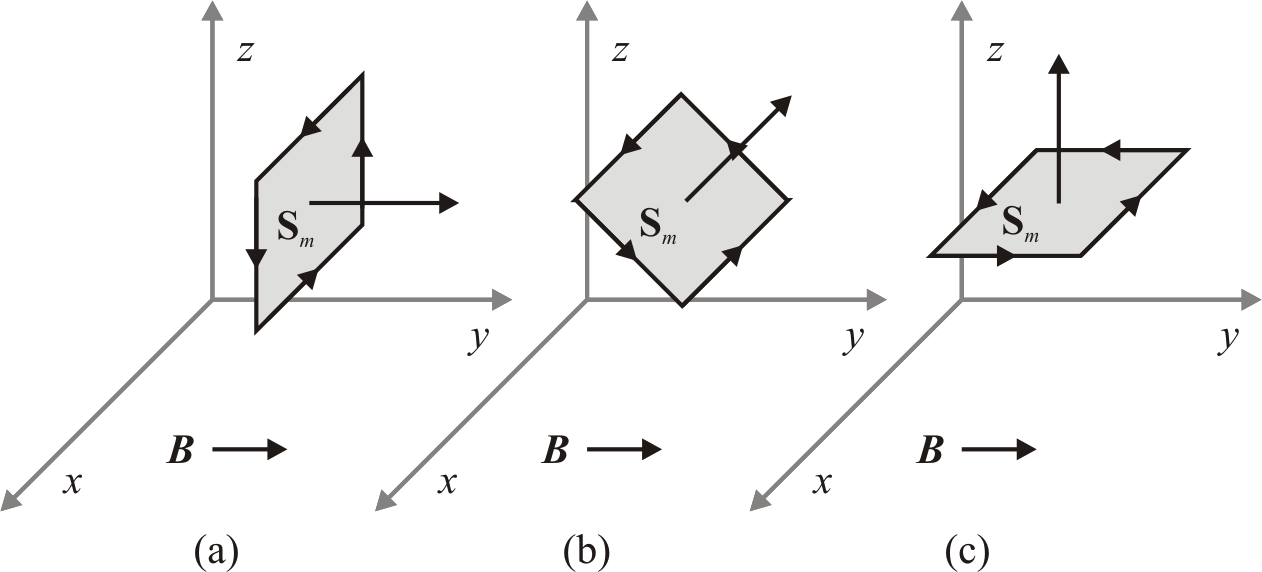
\includegraphics[width=.9\linewidth]{./flux.png}
\end{center}

\section{Gauss's Law and Kirchoff's Flux Law}
\label{sec:org8314f68}

Since there are no magnetic monopoles, we have $$\oint B \cdot \overrightarrow{dS} = 0$$ (Gauss's Law)

Written another way, using the relation from before: \(\sum \phi = 0\) (Kirchoff's Flux Law)

\section{Relation to Ohm's Law}
\label{sec:orgbc090c4}

\(F = \phi \underbrace{R}_\text{reluctance}\)

\section{DC Machines}
\label{sec:org5bf748a}
Some DC machines have two separate electrical systems.

\section{Field Winding}
\label{sec:org9777dbb}
\section{Armature Winding}
\label{sec:orgd369a5e}
The voltage across the armature winding can be given by 

$$v_a = i_a r_a + \text{coil EMF} = i_a r_a + \frac{d}{dt} L_{aa}$$

\section{Field Energy and Coenergy}
\label{sec:org361bb91}
\section{Force}
\label{sec:orge858de4}
force: \(f_e = - \frac{dW_f(\lambda, x)}{dx}\)

force: \(f_e = \frac{dW_c(\i, x)}{dx}\)

\section{Useful Relations}
\label{sec:org233e2bc}

\textbf{reluctance} : \(R = \frac{l}{A \mu}\ \text{H}^{-1}\), where \(l\) is length, \(A\) is area, and \(\mu\) is permittivity
  note that \(\mu\) is not always constant and can depend on conductor current

\textbf{flux} : $$\phi = \frac{Ni}{R} = \int_A \overrightarrow{B} \cdot d \overrightarrow{S}$$, where \(N\) is the number of loops, \(i\) is the current, \(R\) is reluctance, \(B\) is the flux density, and \(A\) is the cross sectional area

\textbf{flux linkage} : \(\lambda = N \phi = Li\), where \(N\) is the number of loops

\textbf{MMF drop} : $$F = Ni = \phi R = \oint \overrightarrow{H} \cdot d \overrightarrow{l}$$

\(V = \frac{d \lambda}{dt}\)

\textbf{co energy} : $$W_c = \left[ \int_{0}^{i_{1,f}} \lambda_1 di_1 \right]_{\substack{i_2 = 0 \\ ...}} + \dots + \left[ \int_{0}^{i_{n,f}} \lambda_n di_n \right]_{\substack{\dots \\ i_{n-1} = i_{n-1,f}}} = \frac{1}{2} i^T L i$$

\textbf{conservative system} : $$\left[ \begin{matrix} \lambda_1 \\ \vdots \\ \lambda_n \end{matrix} \right] = \underbrace{\left[ \begin{matrix} L_{11} & \dots & L_{1n} \\ \vdots & \ddots & \vdots \\ L_{n1} & \dots & L_{nn} \end{matrix} \right]}_{\text{inductance matrix}} \left[ \begin{matrix} i_1 \\ \vdots \\ i_n \end{matrix} \right]$$

if the inductance matrix is diagonally symmetric, then the system is conservative because $$\frac{d \lambda_j}{d i_k} = \frac{d \lambda_k}{d i_j}$$

\textbf{force} : $$f_e = \frac{1}{2} \frac{dL}{dx} i^2$$
\textbf{torque} : $$T_e = \frac{1}{2} \frac{d \lambda}{d \theta_r} i^2$$

nick north : $$\frac{(\overrightarrow{H} \times \overrightarrow{C}) \times \hat{z}}{\left|(\overrightarrow{H} \times \overrightarrow{C}) \times \hat{z}\right|}$$
\end{document}
